\typeout{}\typeout{If latex fails to find aiaa-tc, read the README file!}
%


\documentclass[]{aiaa-tc}% insert '[draft]' option to show overfull boxes
\usepackage{subfigure}
\usepackage{url}


 \title{Development of a Small Bipropellant Rocket Engine Utilizing Additive Manufacturing Processes}


 \author{
  John Tucker%
    \thanks{Student, Maseeh College of Engineering, AIAA Student Member.}
    \ Tamara Dib\thanksibid{1}\
  \ Taylor Rice\thanks{Student, Maseeh College of Engineering, AIAA Member}\ 
  \ Erin Schmidt\thanksibid{1}\
  \ Kristin Travis\thanksibid{1}\\
  \and
  \ and Bianca Viggiano%
   \thanks{Student, Maseeh College of Engineering.}\\
  {\normalsize\itshape
 Portland State University, Portland, OR, 97201, United States}
 }
 
 \AIAApapernumber{YEAR-NUMBER}
 \AIAAconference{AIAA SPACE 2016, 13-16 September 2016, Long Beach, California}
 \AIAAcopyright{\AIAAcopyrightD{2016}}

 % Define commands to assure consistent treatment throughout document
 \newcommand{\eqnref}[1]{(\ref{#1})}
 \newcommand{\class}[1]{\texttt{#1}}
 \newcommand{\package}[1]{\texttt{#1}}
 \newcommand{\file}[1]{\texttt{#1}}
 \newcommand{\BibTeX}{\textsc{Bib}\TeX}

\begin{document}

\maketitle

\begin{abstract}
The complexity and cost of building a liquid fuel rocket engine typically makes such devices unobtainable for a majority of parties interested in their construction. Until recently, manufacturing processes and techniques limited the geometries available to the designer and rendered such engines cost prohibitive as options for inexpensive orbital space flight. Advances in additive manufacturing technologies provide the potential to prototype complex geometries on a lower budget and with lead times which would be considered unobtainable with traditional manufacturing methods. Furthermore, bipropellant liquid fuels offer many complex engineering considerations; the full analysis of which may not be within the design ability of many amateur builds. It is therefore advantageous to develop techniques for additive manufacturing rapid prototyping to make the study of bipropellant fuels more accessible. A mechanical engineering senior capstone team at Portland State University developed an open-source method for quickly prototyping small bipropellant liquid fuel rocket engines with regenerative and film cooling using additive manufacturing.
\end{abstract}





\section*{Nomenclature} %keeping dummy variables for guidance

\begin{tabbing}
  XXXXX \= \kill% this line sets tab stop
  $PSAS$ \> Portland State Aerospace Society\\
  $DMLS$ \> Direct Metal Laser Sintering\\
  $LFRE$ \> Liquid Fuel Rocket Engine\\
  $LOX$ \> Liquid Oxygen\\
  $AM$ \> Additive Manufacturing\\
  $BF$ \> Blockage Factor\\
  $TMR$ \> Total Momentum Ratio\\
  
 % $\Delta x$ \> Variable displacement vector \\
 % $\alpha$ \> Acceleration, m/s\textsuperscript{2} \\[5pt]
 % \textit{Subscript}\\
 % $i$ \> Variable number \\
 \end{tabbing}


\section{Introduction}
The Portland State Aerospace Society (PSAS) is an engineering student group dedicated to low-cost, open-source technology development for high powered rockets and avionics systems \cite{PSAS}. The stated long term goal of the group is to place a 1 $kg$ CubeSat into low Earth orbit with their own launch vehicle. One step needed to achieve this goal is to transition the current rocket design from a solid to liquid fuel engine. Explored herein is the process of designing and testing a 500 $lbf$ thrust engine using liquid oxygen (LOX) and ethanol as propellants with regenerative cooling channels, film cooling, and a pintle injector. The design process is documented using Python in Jupyter notebooks and shared using Github \cite{git}. The authors feel that open standards for space systems hardware and design will be of increasing importance to the nascent `new space' industry. In this context, and in the interest of empowering `citizen scientists' and raising the level of public discussion on the issue of low-cost access to space the (non-ITAR controlled), project deliverables are being made freely and publicly available under a GNU GPL v3.0 open-source licence. 

A Jupyter Notebook is a sharable web application which allows for the live execution of code, namely Python. Jupyter notebooks were utilized in order to create a development process for the design of a regeneratively and film cooled liquid fuel rocket engine. The Jupyter Notebook forms a template for regeneratively cooled chamber design. As design inputs are changed in the notebook, parametric curves, which form the basis of the geometry file for 3D printing, are generated appropriately. This allows for quicker development of geometry files for additive manufacturing and thus quicker lead times on engine prototyping. As additive manufacturing technology progresses and becomes widely accepted by industry, its capability in rocket component design needs to be further studied and understood. Alloys used in Direct Metal Laser Sintering (DMLS) have different strength, heat transfer, and surface roughness properties. This project aims to gain insights on these properties and 3D printed combustion chamber performance. 


% it would appear we've covered everything without a top level design section, should we move things out of engine? or will this be sufficient?

%\section{Top Level Design}


\section{Engine}

%make the table a sub section? Also, i have zero clue about the style guide for a table, so I'm just going to construct it, with as much information as possible, we can cut or add anything we want, and style it all at once. I've commented out a lot of engine parameters, if you want to include them just uncomment them.


Engine design is typically cost prohibitive for many amateur designers who may be able to contribute to the advancement of low cost orbital space flight. The design process is cumbersome, and oftentimes does not result in a final product that will successfully fire due to the complexity of engine design. Engineering tools are not generally available, and an understanding of the full process is lacking. Due to the aforementioned constraints, it is desirable for the amateur to have available a design tool which will aid in generating a geometry capable of withstanding the stresses of a steady-state engine, while simultaneously producing a desired thrust. A production engine was generated and built using the Jupyter Notebook. Table \ref{tab:engineparams} shows a variety of the theoretical engine parameters generated by the liquid fuel rocket engine (LFRE) notebook.

\begin{table}
\begin{center}
\begin{tabular}{| l | c | c |}

\hline
 Parameter, variable                      & Unit     & Value     \\
 \hline
 Nozzle force, $F$                        & $lbf$       & 500       \\
 O/F weight mixture ratio, $r_w$          & --  & 1.2       \\
 Fuel mixture percentage, $r_{w_{fuel}}$  & --   & 0.595      \\
 Contraction ratio, $\varepsilon_c$       & --  & 10.5      \\
 Ratio of specific heats, $\gamma$        & --  & 1.12      \\

 %Pressures:
 Total chamber pressure, $P_{c_{inj}}$    & $psi$  & 350.00    \\
 Throat pressure, $P_t$                   & $psi$       & 202.73    \\

 %Velocities:
 Throat velocity, $V_t$                   & ${ft}/{s}$    & 3464.05   \\
 Exit velocity, $V_e$                     & ${ft}/{s}$    & 7804.45   \\

 %Mass Flow Rates:
 Total mass flow rate, $\dot w$           & ${lb}/{s}$    & 2.06      \\

 %Temperatures:
 Stagnation temperature, $T_{c_{ns}}$             & $^\circ R$ & 5487.10   \\
 Adiabatic wall temperature at inlet, $T_{awi}$   & $^\circ R$ & 4389.64   \\
 Adiabatic wall temperature at throat, $T_{awt}$  & $^\circ R$ & 4379.47   \\

 Specific Impulse, $I_s $                 & ${lb\cdot s}/{lb}$    & 242.37    \\
 Characteristic velocity, $c*$            & ${ft}/{s}$            & 5325.59   \\

 Chamber volume, $V_c$                    & $in^3$      & 27.35     \\
 Chamber cross sectional area, $A_c$      & $in^2$      & 10.26     \\
 Throat radius, $r_t$                     & $in$        & 0.558     \\
 Exit radius, $r_e$                       & $in$        & 1.037     \\
 Wall thickness, $t$                      & $in$        & 0.01820   \\
 
 Cooling channel base width at throat, $b_t$              & $in$        & 0.02522   \\
 Cooling channel base width at exit, $b_e$                & $in$        & 0.06192   \\
 Cooling channel effective radius at throat, $r_{cch_t}$  & $in$        & 0.01261   \\
 Cooling channel effective radius at exit, $r_{cch_e}$    & $in$        & 0.03096   \\
 Cooling channel hydraulic diameter, $d$                  & $in$        & 0.04671   \\
 Cooling channel total area, $A_c$                        & $in^2$      & 1.16537   \\
 Number of cooling channels, $n$                          & --  & 82        \\

 Coolant side heat transfer coefficient, $h_c$    & ${Btu}/({in^2\cdot s\cdot^{\circ}F})$   & 0.15609   \\
 Required heat flux, $\dot q$                          & ${Btu}/({in^2\cdot s})$                 & 27.72     \\
 Coolant capacity, $Q_c$                          & ${Btu}/{s}$                           & 341.68    \\
 
 Combined tangential stress at nozzle exit, $S_{t_e}$     & $psi$       & 32224.43  \\
 Combined tangential stress at throat, $S_{t_t}$          & $psi$       & 31554.40  \\
\hline
\end{tabular}
\end{center}
\caption{Parameters obtained from the Jupyter Notebook for the production engine chamber and nozzle design.}
\label{tab:engineparams}
\end{table}

The LFRE Nozzle Jupyter Notebook \cite{LFRE} allows the user to input desired design requirements; namely thrust and material properties, to subsequently aid the designer in generating an acceptable geometry for the specified requirements. NASA's CEARUN tool \cite{CEARUN} is used to generate many of the initial design parameters as inputs. Certain design constraints (fuel combination, mixture ratio, and chamber pressure) must be known prior to utilizing the CEARUN tool, and should be selected according to needs of the engine design. After inputs are provided, the basic geometry of the nozzle is determined. Furthermore, the analysis determines the cooling capacity of the fuel used in regenerative passages resulting in parametric equations which describe the chamber and nozzle contours, the inner and outer surfaces of the regenerative cooling passages, and the external surface of the nozzle. The parametric equations may then be used to generate a printable 3D model in combination with additive manufacturing processes.

The regenerative cooling passages constructed using the parametric equations are of uniform cross-sectional area normal to the surface of the nozzle contour. These parametric equations were derived in order to mathematically define a nozzle contour and its various cooling channel geometries in general such that no geometry would have to be calculated by the designer, and a nozzle could be generated by virtue of only the geometric parameters which make it unique \cite{parametricEQs}. Full development of the parametric equations are available for inspection, but are not provided here for the sake of brevity. This allows the  cross sectional area to be scaled as a means of controlling the velocity of the fuel in a particular regenerative passageway, enabling better control of wall temperatures at any given axial position along the nozzle. Scaling functions may be added as a design tool at a later date, but initial functions resemble a half period of a sine function to scale along a desired length of nozzle in order to give a smooth and continuous scaling pattern along a given section of the nozzle. Because the nozzle is parametrized, any parametric equation justifying a nozzle section may simply be multiplied by a scaling function in order to more directly control cooling over specific areas of the nozzle.
 
After generating parametric equations, a more detailed heat transfer analysis is undertaken. Properties are evaluated along finite sections of the wall contour, and compared to the capacity of the specified coolant, to allow the designer to analyze if a particular nozzle geometry is capable of reaching a thermal equilibrium while remaining below the thermal and mechanical stress limits of the engine material and the boiling point of the fluid. The analysis generates graphs of several key properties along the nozzle contour as shown in figure \ref{fig:propertygraphs}. The major outputs of the Jupyter Notebook are a unique set of parametric equations with which a liquid fuel rocket engine is created which utilizes regenerative and film cooling to protect the engine material from yield due to thermal and mechanical stresses during thermally steady state combustion.

%\begin{figure}[h]
%\centering
%   {\includegraphics[width=.3\textwidth]{graphs/radius_v_position.png}
%    \includegraphics[width=.3\textwidth]{graphs/mach_v_position.png}
%    \includegraphics[width=.3\textwidth]{graphs/pressure_v_position.png}
%    \includegraphics[width=.3\textwidth]{graphs/temp_v_position.png}
 %   \includegraphics[width=.3\textwidth]{graphs/velocity_v_position.png}
 %   \includegraphics[width=.3\textwidth]{graphs/HT_coeff_v_position.png}
 %   \includegraphics[width=.3\textwidth]{graphs/adiab_wall_temp_v_position.png%}
 %   \includegraphics[width=.3\textwidth]{graphs/heat_flux_v_position.png}}
 %   \caption{LFRE Jupyter Notebook sample output for various properties along the length of the developed nozzle}
 %%   \label{fig:propertygraphs}
%\end{figure}

\begin{figure}[ht]
\centering
   {\includegraphics[width=.3\textwidth]{figures/mach}
    \includegraphics[width=.3\textwidth]{figures/temp}
    \includegraphics[width=.3\textwidth]{figures/hx}}
    \caption{LFRE Jupyter Notebook sample output for Mach number, temperature and heat flux along the length of the developed nozzle. For a complete set of parameters plotted as a function of nozzle position see the Github repo \cite{LFRE}.}
    \label{fig:propertygraphs}
\end{figure}


Correction factors are implemented into the Jupyter Notebook to address discrepancies between theoretical values for various parameters and their empirically tested values. The primary correction factor to be addressed after testing an engineering prototype should be the adiabatic wall temperature of the hot exhaust gas due to film cooling. Models for film cooling are not well established, and it is important to determine a correction factor for a particular engine in order to accurately predict the resulting physical properties of subsequent iterations of engine prototypes. This will allow a designer to predict the flow rates and pressure drops of propellants with enough accuracy to design a propellant feed system capable of delivering required pressure to an engine without the need to iterate through many costly test stand designs.


\subsection*{Engine Features}

The first engine prototype shown in figure \ref{fig:nozzlecross} is intended to produce 500 $lbf$. It is produced by a DMLS 3D printing process and made from high temperature aluminum alloy, AlSI10Mg. External to this project, a test stand  is being built that is capable of delivering fuel at approximately 500 $psi$ to the fuel manifold, which is located at the base of the nozzle bell. Upon collection, the fuel is directed through regenerative cooling channels. The fuel is then delivered to a collection chamber. Care should be taken to limit the overhang angles within the larger geometries of the collection chamber. This limit is dictated by the particular 3D printing process which is being utilized. The designer should consider the print orientation and maximum overhang angle. The presented prototype was printed with a maximum overhang angle of 45$^\circ$, and the design resulted in minimal use of support material. Upon collection, the fuel is directed to film cooling ports, shown in figure \ref{fig:designcross}; of which the size and quantity are optimized by the Jupyter Notebook. Remaining fuel is then utilized as propellant, which is directed around a pintle injector, described in section \ref{sec:PI}. After injection and combustion occur, the propellants are directed through a de Laval nozzle design based on Rao's parabolic bell approximation \cite{rao1961recent}.

\begin{figure}[ht]
\centering
   {\includegraphics[width=.85\textwidth]{nozzlecross}}
    \caption{Final assembly cross section drawing of the rocket engine. Areas in red show the regenerative cooling channels and the path the fuel takes through the engine. Areas in green are the liquid oxygen flow path.}
    \label{fig:nozzlecross}
\end{figure}


\begin{figure}[ht!]
\centering
    {\includegraphics[width=.65\textwidth]{designcross}}
    \caption{Final design cross section drawing of the nozzle bell, the nozzle and fuel manifolds are manufactured as a single part. The nozzle is a parabolic approximation of a de Laval converging-diverging nozzle.}
    \label{fig:designcross}
\end{figure}

DMLS uses high energy pulse CO2 lasers (carbon dioxide laser) to fuse metal particles together, layer-by-layer, to form a solid product. The process is done in a powder bed that inherently provides support material for any overhanging features. Because of this, complex features and internal passageways are possible utilizing DMLS that are not possible with traditional machining approaches. Incorporating DMLS manufacturing allows the designer to work towards the 'ideal' design for a rocket engine without the added burden of considering machinability. Features such as regenerative cooling channels no longer require special machining strategies for incorporation into a design. They are instead printed directly into the nozzle contours simply and accurately with only feature size and overhang angles as constraints. 

\section{Pintle Injector}
\label{sec:PI}

%The pintle section needs a stats table, similar to the engine stats table. 
%Here it is, but it needs formatting

There are several possibilities for the selection of the injector.
%This sentence doesn't make sense to me. Are 'stable and efficient manners' performance characteristics? Which performance characteristics?
%Most injector types are capable of atomizing the fuel in a stable and efficient manner, therefore performance characteristics are not the driving factor in design selection.
A 500 $lbf$ thrust engine has low fuel mixing requirements; as long as the mass flow rates and momentum ratios are satisfied, many different designs will suffice. Swirl injectors, as well as impinging jet injectors were considered; however, these designs are more complex and potentially more difficult to integrate with 3D printed cooling channels. As a result, an interchangeable pintle injector design based on 
research published by Santoro was selected \cite{santoro1999main}. A pintle injector will be fixed to the engine via bolts or machine screws, making it relatively easy to remove and replace if alterations are necessary. Additionally, pintle injectors are less susceptible to combustion instabilities  and are potentially throttle-able; features that will benefit future PSAS liquid engine designs\cite{dressler2000trw}. 
%is it ok that I changed 'larger' to 'PSAS liquid'?


The pintle injector is responsible for delivering the liquid oxygen to the combustion chamber. 316 stainless steel was chosen as the pintle injector material because of its LOX compatibility and thermal resistance qualities. The liquid oxygen travels down the center of the pintle and leaves the LOX holes at a 90$^\circ$ angle to the original direction of travel. The liquid oxygen exiting the pintle holes collides with the annulus fuel stream and creates an atomized mixture. The oxygen holes and fuel gap have been sized to achieve near equal flow momentum of each propellant resulting in a TMR near unity to ensure the trajectory of the mixture inside the combustion chamber is $\sim$45$^\circ$. The design for the pintle injector is shown in figure \ref{fig:PIxsection}.

\begin{figure}
\centering
   \subfigure[]{\includegraphics[width=.45\textwidth]{PintleDims}}
   \subfigure[]{\includegraphics[width=.45\textwidth]{PintleRoundIso}}
    \caption{Pintle LOX holes and fuel annulus inside combustion chamber (a) and Stainless Steel pintle injector design (b).}
    \label{fig:PIxsection}
\end{figure}

Currently there is little published data on the design and construction of pintle injectors. Therefore an extensive documentation of the design process has been outlined in the Github repository. Using the Jupyter Notebook in Github, radii for the LOX holes and the fuel annulus were determined from inputs for required chamber pressure and propellant mass flow rates. The dimensions of the radii can be adjusted according to recommended blockage factor (BF) and total momentum ratio (TMR) values provided by Woodward \cite{woodward1998injector}. The notebook is constructed for ease in calculations for an iterative process. Table \ref{tab:pintle} shows the theoretical parameters generated by the Jupyter Notebook that pertain to the design of the current pintle injector.

\begin{table}
\begin{center}
\begin{tabular}{| l | c | c |}
\hline
 Parameter, variable                          & Unit     & Value     \\
  \hline
  Pintle center LOX flow rate, $\dot w_{ox}$                                  & ${lb}/{s}$       & 1.13       \\
   Outer annulus ethanol flow rate, $\dot w_f$
   & ${lb}/{s}$       & 0.94       \\
 Pintle outer radius, $R_p$                              & $in$       & 0.14       \\
 Pintle inner radius, $r$          
 & $in$   & 0.06       \\
Fuel annulus radius, $R_a$          
 & $in$   & 0.152       \\
 Annulus gap, $t$          
 & $in$   & 0.012       \\
 Injector pressure drop, $\Delta P$          
 & $psi$   & 70       \\
  Pintle hole diameter, $d_h$          
 & $in$   & 0.045       \\
   Number of pintle LOX holes, $N$         
 & --   & 8       \\
  Theoretical Blockage Factor, $BF$          
 & --   & 0.41       \\
   Theoretical Total Momentum Ratio, $TMR$          
 & --   & 0.97       \\  
\hline
\end{tabular}
\end{center}
\caption{Parameters obtained from the Jupyter Notebook for the current pintle injector design.}
\label{tab:pintle}

\end{table}

\section{Ongoing and Future Work}
All entities of the printed production engine, shown in figure \ref{fig:IMG_1371}, must still be tested, including the injector and nozzle. The regenerative cooling channels of the nozzle will be cold flow tested prior to any hot fires. The pintle injector has been designed and is in the midst of being machined; it will be cold flow tested prior to being attached to the nozzle. The ignition system is currently being designed as well as the instrumentation to test fire the engine.%'engine' used to be 'rocket'. 

\begin{figure}[ht!]
\centering
    {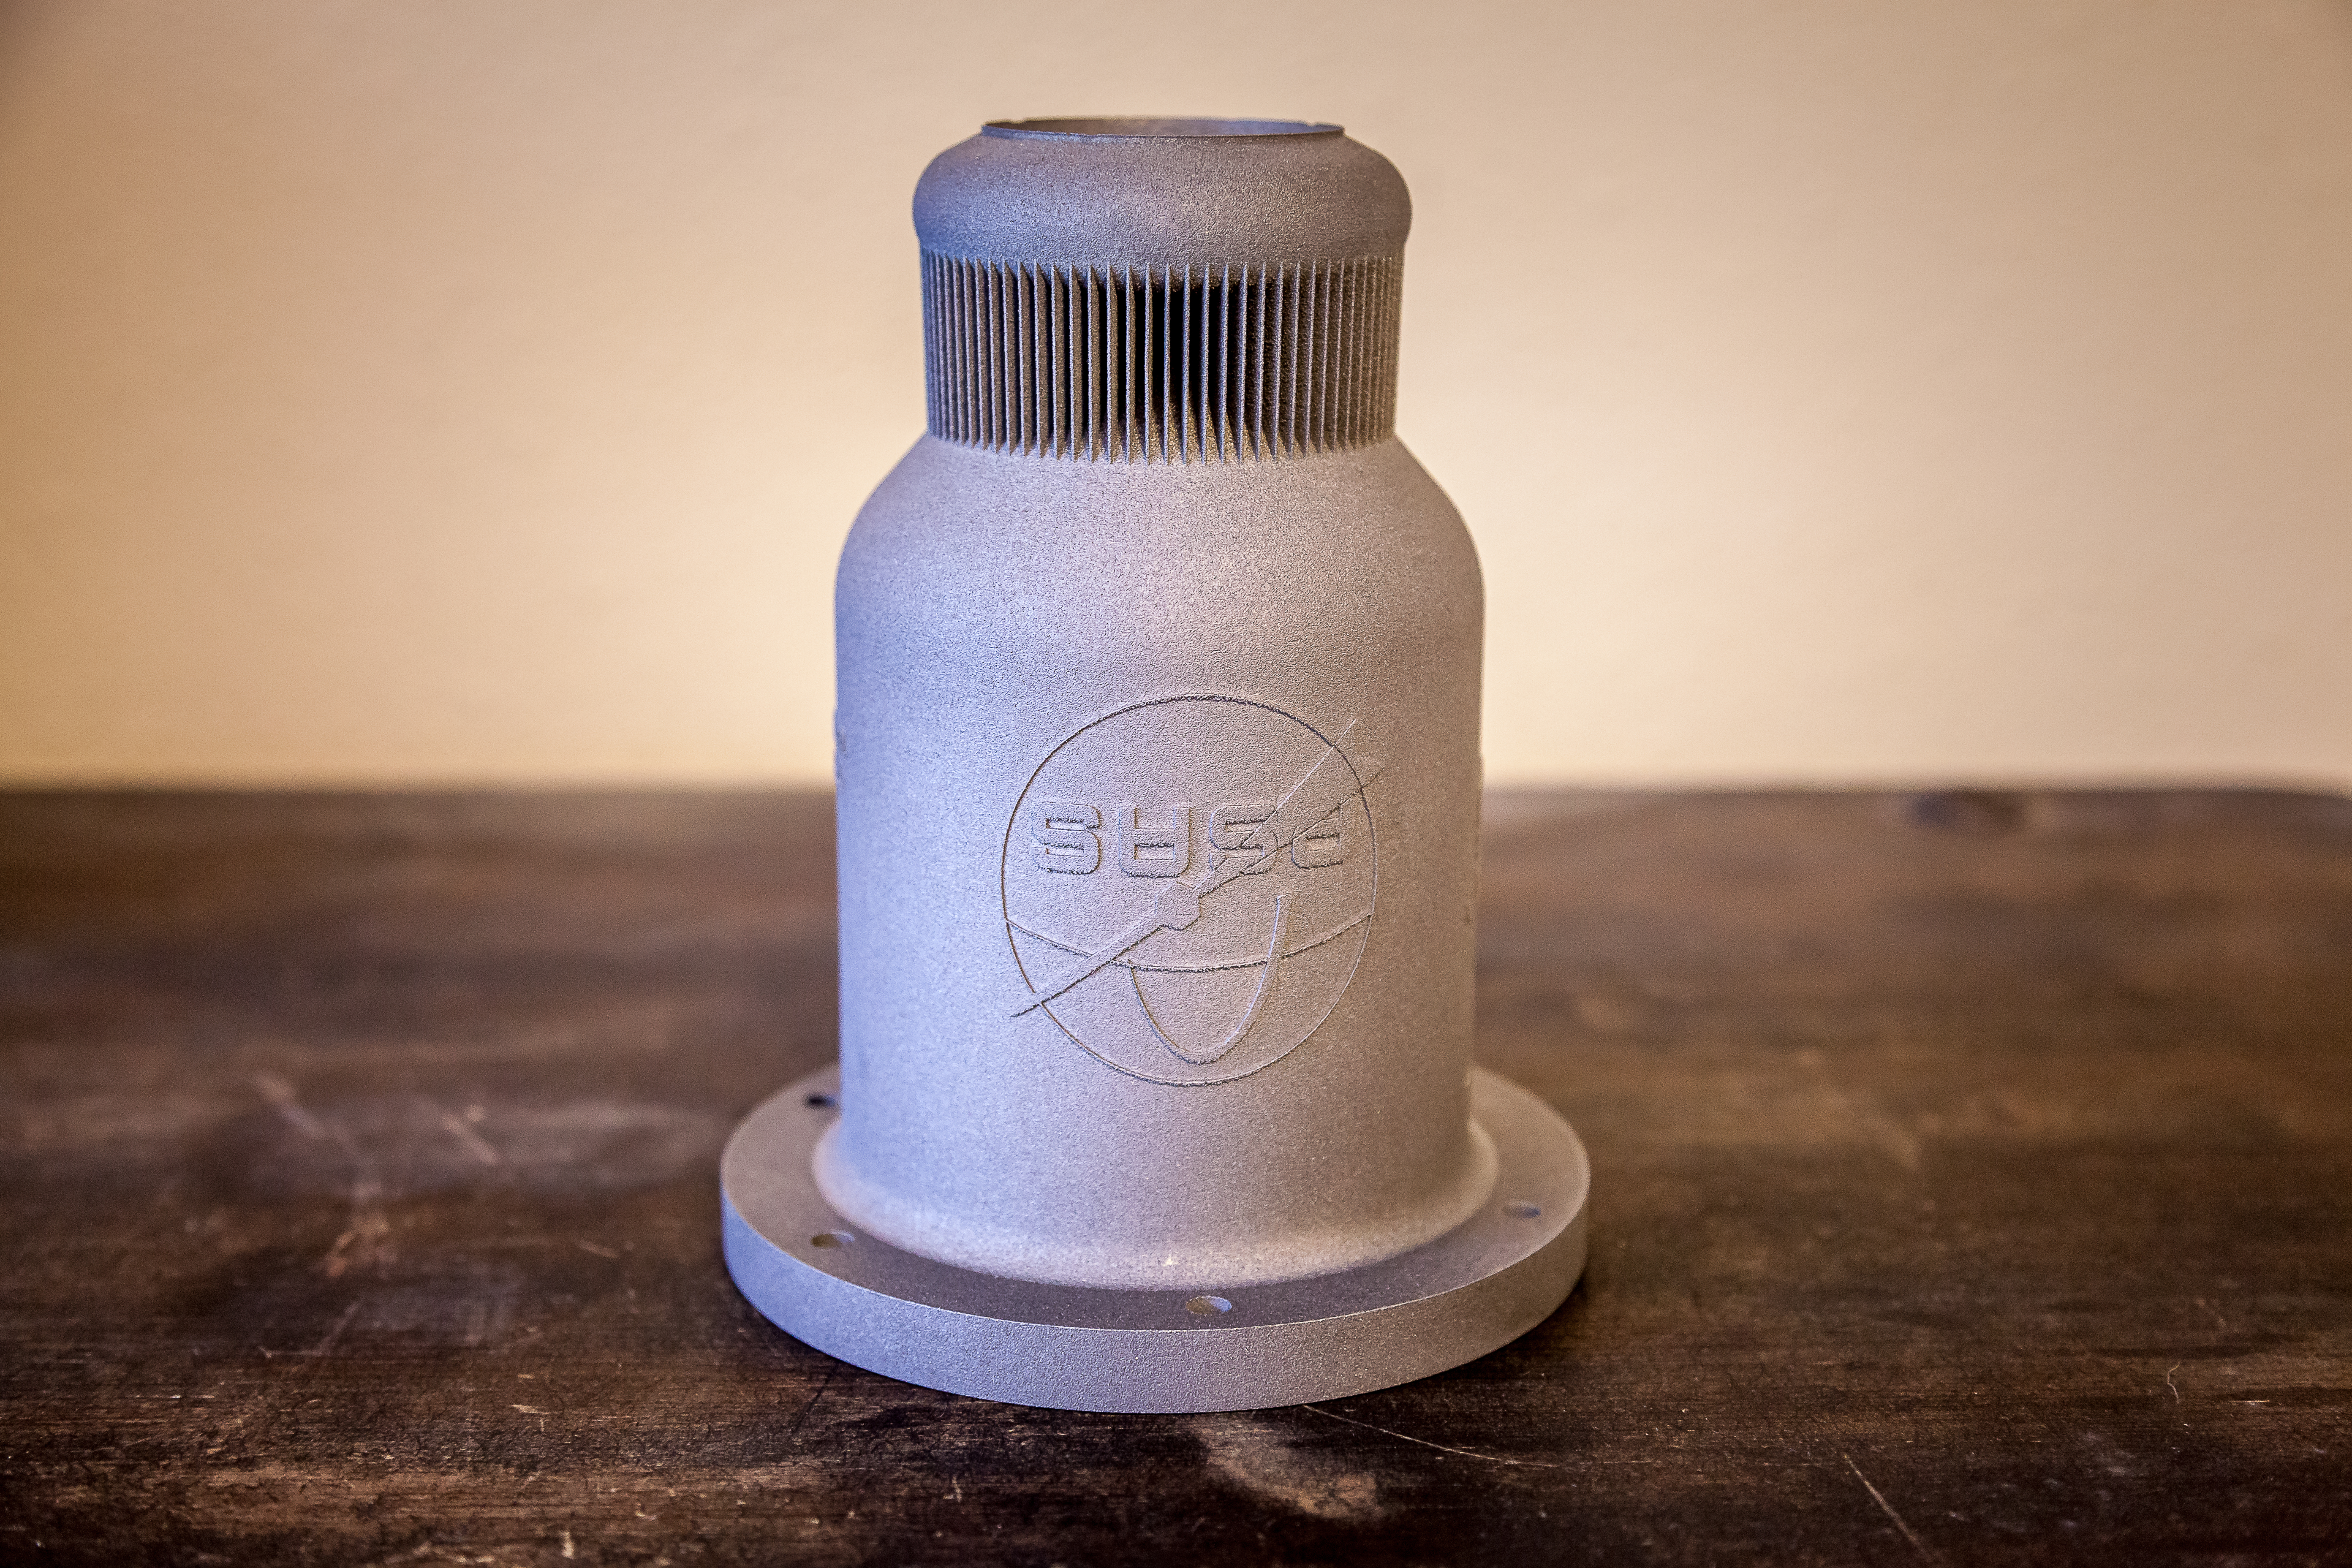
\includegraphics[width=.65\textwidth]{IMG_1371}}
    \caption{Printed engine to be cold tested and hot fired.}
    \label{fig:IMG_1371}
\end{figure}


A future iteration of the Jupyter Notebook would include constant hydraulic diameter as an output rather than a constant cross sectional area, in order to give the designer a unit flow velocity along the channels. The flow velocity could then be scaled as desired around areas of high heat transfer such as the throat.


\section{Conclusion} %I am adddding a sentence here.
To the knowledge of the authors, no other open-source method for quickly prototyping liquid fuel engines exists. The first iteration of this engine will be tested on a test stand in 2016. The results obtained from the cold tests and hot fire of the engine will aid in future iterations and give insight into the validity of the equations utilized for this engine. 3D printed engines are just beginning to be developed and tested by industry, and few have been tested in flight. Additive manufacturing has opened the door for design innovation, low cost development, and amateur group access to space.



%\section*{Appendix}
%should we include links to things like the derivations of contour equations, or the various Jupyter notebooks?



\section*{Acknowledgments}
The authors are grateful to PSAS for funding and initiating this project, Faculty Advisor Dr. Derek Tretheway for his advice and guidance and Cam Yun for his work on the project. The authors are also grateful to Robert Watzlavick, David Gregory, and Armor Harris for their advice, and the Oregon Air National Guard for their guidance on LOX handling. Finally the authors are indebted to i3D MFG for their ongoing support with additive manufacturing and Machine Sciences Corporation for their support with traditional machining.

\bibliography{aiaabib}
\bibliographystyle{aiaa}


\end{document}